% Kopfzeile beim Kapitelanfang:
\fancypagestyle{plain}{
%Kopfzeile links bzw. innen
\fancyhead[L]{\calligra\Large Vorlesung Nr. 16}
%Kopfzeile rechts bzw. außen
\fancyhead[R]{\calligra\Large 05.12.2013}
}
%Kopfzeile links bzw. innen
\fancyhead[L]{\calligra\Large Vorlesung Nr. 16}
%Kopfzeile rechts bzw. außen
\fancyhead[R]{\calligra\Large 05.12.2013}
% **************************************************
%
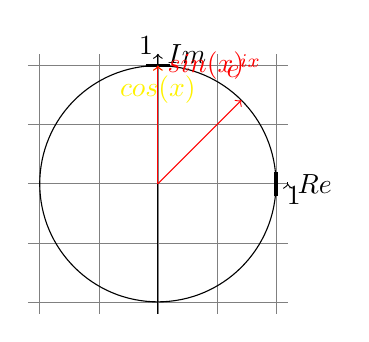
\begin{tikzpicture}[domain=-1.2:1.2, scale=1.5, prefix="plots/", smooth]
	% Raster einzeichnen
    \draw[very thin,color=gray,step=0.5] (-1.1,-1.1) grid (1.1,1.1);
    % Koordinatensystem
    \draw[->] (1.1, 0) -- (1.1,0) node[right] {$Re$}; 
    \draw[->] (0, -1.1) -- (0,1.1) node[right] {$Im$};
    \draw[-, very thick]  (1, 0.1) -- (1, -0.1) node[below, right] {1};
    \draw[-, very thick]  (0.1, 1) -- (-0.1, 1) node[left, above] {1};
    % Einheitskreis zeichnen
    \draw[color=black] (0,0) circle (1);
    % Pfeil einzeichnen
	\draw[<-,color=red] (45:1)++(0,0) -- (0,0);
	\draw[color=red] (0.5,1) node[right] {$e^{ix}$};
	\draw[->,color=yellow] (0,0)--(0,1) node[below] {$cos(x)$};
	\draw[->,color=red] (0,0)--(0,1) node[right] {$sin(x)$};
\end{tikzpicture}
\chapter{Stetige Funktionen und Grenzwerte}
Sei $D \subseteq \R, f:D\to\R$ Funktion\\
Varianten:\\
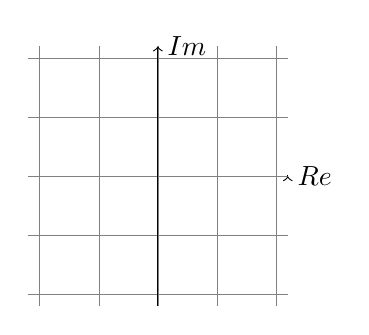
\begin{tikzpicture}[domain=-1.2:1.2, scale=1.5, prefix="plots/", smooth]
	% Raster einzeichnen
    \draw[very thin,color=gray,step=0.5] (-1.1,-1.1) grid (1.1,1.1);
    % Koordinatensystem
    \draw[->] (1.1, 0) -- (1.1,0) node[right] {$Re$}; 
    \draw[->] (0, -1.1) -- (0,1.1) node[right] {$Im$};
	%todo Stetige Funktion mit x_0-\delta und x_0+\delta (schraffierter Bereich)
\end{tikzpicture}
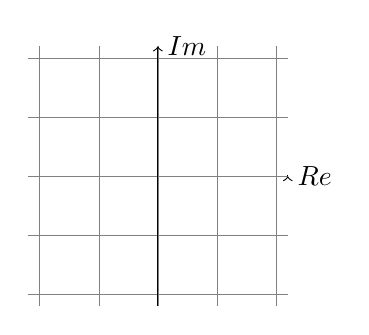
\begin{tikzpicture}[domain=-1.2:1.2, scale=1.5, prefix="plots/", smooth]
	% Raster einzeichnen
    \draw[very thin,color=gray,step=0.5] (-1.1,-1.1) grid (1.1,1.1);
    % Koordinatensystem
    \draw[->] (1.1, 0) -- (1.1,0) node[right] {$Re$}; 
    \draw[->] (0, -1.1) -- (0,1.1) node[right] {$Im$};
	%todo unstetige Funktion
\end{tikzpicture}
\section{Definition: Stetigkeit}
Sei $D \subseteq \R, f: D\to\R$ Funktion\\
$f$ heißt \ul{stetig} in $x_0 \in D \Leftrightarrow \forall \e > 0 \exists \delta>0: |f(x) - f(x_0)|<\e$ für alle $x\in D$ mit $|x - x_0|<\delta$\\
($\e - \delta$-Kriterium)\\
$f$ stetig auf $D \Leftrightarrow f$ stetig in jedem $x_0\in D$\\
Interpretation\\
%TODO Schaubild
Kleine Änderungen der Eingabe bewirken nur kleine Änderungen der Ausgabe.
\section{Folgenkriterium}
Für $f:D\to \R$ gilt:\\
$f$ stetig in $x_0 \in D \Rarr $ für jede Folge $(x_n|\subseteq D$ mit $x_n\to x_0$ gilt $\lim\limits_{n\to ∞} f(x_n) = f(x_0)$)\\
$\e - \delta$-Definition der Stetigkeit in $x_0$:\\
$\forall \e > 0 \exists \delta>0:|f(x) -f(x_0)|<\e \forall x\in D$ mit $|x-x_0|<\delta$\\
Beweis $\Rarr$\\
Sei $(x_n) \subseteq D$ mit $x_n \to x_0$.\\
Sei $\e > 0 \overset{\e - \delta-Krit.}{\Rarr} \exists \delta > 0$\\
$|f(x_n) - f(x_0)|< \e$ sofern $|x_n - x_0|<\delta$\\
$\lim\limits_{n\to ∞}x_n = x_0 \Rarr \exists n_0 \in \N:|x_n - x_0|< \delta \forall n ≥ n_0$\\
Also $|f(x_n) - f(x_0)| < \e\forall n ≥ n_0 \Rarr f(x_n) \to f(x_0)$\\
Beweis $\Leftarrow$\\
Angenommen f sei unstetig in $x_0$. Dann $\exists \e_0>0$ zu dem sich kein $\delta$ finden lässt, so dass $\e-\delta-$Kriterium erfüllt ist.\\
Insbesondere zu $\frac{1}{n} - \delta (n\in \N) \exists x_0 \in D:|x_n - x_0|< \frac{1}{n}$, aber $|f(x_n) - f(x_0)|>\e_0$\\
Also $x_n \to x_0$ aber $f(x_n)\not\to f(x_0)$\lightning \qed
\section{Regeln für Stetige Funktionen}
Seien $f, g: D \to \R$ stetig in $x_0\in D \Rarr f+g, f\cdot g, c \cdot f~(c\in \R): D\to \R $ sind ebenfalls stetig in $x_0$.\\
Dabei gilt 
\enum{
\item $f(x) + g(x) = (f+g)(x)$
\item $(c\cdot f)(x) = c \cdot f(x)$
}
Falls $g(x_0) \neq 0 \Rarr \frac{f}{g} : \{x\in D: g(x)\neq 0\} \to \R$ ist stetig in $x_0$\\
Beweis:\\
Mit Folgenkriterien und Regeln für Grenzwerte:\\
Sei $(x_n) \subseteq D$ mit $x_n\to x_0$\\
$\Rarr f(x_n) \to f(x_0), g(x_n) \to g(x_0)$\\
$\Rarr f(x_n) + g(x_n) \to f(x_0) + g(x_0) \Rarr f+g$ stetig in $x_0$
\section{Beispiele: Polynome und rationale Funktionen}
\enum{
\item Sei $p(x) = a^nx_n + ... + a_1x + a_0 \in \P_\R$ Polynomfunktion wiederholte Anwendung von 9.3 $\Rarr p$ stetig auf $\R$
\item Eine rationale Funktion auf $\R$ ist eine Funktion der Form:\\
$R(x) = \frac{p(x)}{q(x)}$ mit $p, q \in \P_\R, q\neq 0$\\
Regeln 9.3 $\Rarr R$ stetig auf ganz $D$.\\
Vergrösserung von $D$ eventuell möglich durch Kürzen gemeinsamer Faktoren.
}
\section{Satz}
$exp: \R \to \R, x\to e^x$ ist stetig auf $\R$
\section{Komposition stetiger Funktionen}
Seien $D,E \in \R$ und $f: D \to \R, g: E\to \R$ Funktion mit $f(D) \in E$